\section{Simulations}
\label{sec:sims}

%-------------
\subsection{Cosmic shear galaxy catalogues} 
\label{subsec:WL_cats}

The weak lensing simulations developed for this work are based on  the {\it Outer Rim} $N$-body simulation \citep{OuterRim}, which evolved 10,240$^3$ particles in a $(5.225 \mathrm{Gpc})^3$ cosmological volume, assuming a flat \lcdm cosmology with $\Omega_{\rm m}=0.2648$, $\Omega_{\rm b}=0.0448$, $h=0.71$, $\sigma_8 = 0.801$, $n_{\rm s}= 0.963$, $w_0=-1.00$.
A total of $101$ particle snapshots were originally saved, of which we use only those with $z<3.0$. Particles from each dump are assigned to curved mass shells approximately 114 Mpc thick, producing a sequence of 57 {\sc Healpix} maps $\delta_i(\theta, \phi)$ with {\sc nside} = 8192 and $i=1...57$, filling up a light-cone over an octant up to $z = 3$.
%More details on this procedure can be found  in \citet{cosmoDC}, where lensing quantities are computed specifically for the generation of the {\sc cosmoDC2}  synthetic sky catalogue.

Ray-tracing is performed in the Born approximation, summing over the mass shells using a $\chi$-integral similar to Eq. (\ref{eq:C_ell}), but with only one power of $(q^i/\chi)$ instead of two, and replacing $P_\delta$ with $\delta_i(\theta,\phi)$.
A source plane is placed at the high-redshift edge of every mass planes, resulting in a series of convergence  maps $\kappa_i(\theta,\phi)$ that are subsequently transformed into shear maps $\gamma_{1/2, i}(\theta,\phi)$ using Eq. (\ref{eq:KS}).
We finally position galaxies in the light cone following three distinct algorithm, each impacting the strength of the IA signal:
\begin{enumerate}
\item {\it Random:} galaxies are distributed randomly on the octant, thereby reproducing one of the  fundamental assumptions in the NLA and TT models. 
\item {\it Linear bias:} galaxy positions are sampled from the mass sheets smoothed\footnote{We also tried sampling the field with $0.1$ and $0.5$ $h^{-1}\mathrm{Mpc}$ but this resulted in noisier results.} with a 1.0 $h^{-1}\mathrm{Mpc}$ (comoving) beam, assuming a linear bias of $b_{\rm TA}$, thereby building the one of the key assumptions of the \dNLA and \dTT models. 
We assume $b_{\rm TA}=1.0$ as our fiducial case but also consider $b_{\rm TA}=2.0$ to test  the  model flexibility. 
\item{\it Non-linear bias:} galaxy positions are obtained by populating dark matter haloes with the Halo Occupation Distribution prescription described in \citet{cosmoDC2} and used recently in \citet{TXPipe}\footnote{We used version: {\tt skysim5000\_v1.2}.}. Specifically, we select objects over a patch of 732.20 deg$^2$ given by  0$<$RA$<$ 20 and -36.61$<$DEC$<$0, we apply a magnitude cut of mag$_r<$24.8, and further downsample randomly to retain 20\% of the galaxies, approaching the global galaxy redshift distribution and number density used with the other simulation catalogues (Eq. \ref{eq:nz}).
The sample is further split into 5 tomographic bins by calculating the probability a given galaxy in the HOD sample lies in each bin, based on its true redshift. This is simply done by interpolating each of the tomographic $N(z)$ shown in Fig. 1 at the galaxy?s true redshift, then using these as weights to assign a tomographic bin in a random draw. After a galaxy is assigned, it is removed from the sample to avoid double counting. This method allows us to capture some of the effect of photo-z uncertainty, as it gives all galaxies a small but non-zero probability of being included in tomographic bins outside of their true redshifts. The resulting in the $n(z)$ presented in Fig. \ref{fig:Nz} with the dashed lines, closely matching the target $n(z)$. Compared to the analytical SRD-Y1, the mean redshifts of the five tomographic bins are shifted by [-0.027, -0.018,  0.003, -0.010,  0.038], respectively, which we take into account when making predictions for these HOD lensing mocks.
\end{enumerate}
%Note that while cases (i) and (ii) exactly reproduce the SRD-Y1 $N(z)$ presented in Fig. \ref{fig:Nz} (solid lines), the $N(z)$ in the latter case is not a perfect match, as shown with the dashed lines, although the agreement is good enough for our goal; we return to this in Sec. \ref{subsec:HOD}, where we describe the HOD model and related quantities.  


%----------
\subsection{Projected tidal fields}
\label{subsec:IA_sims}

\begin{figure}
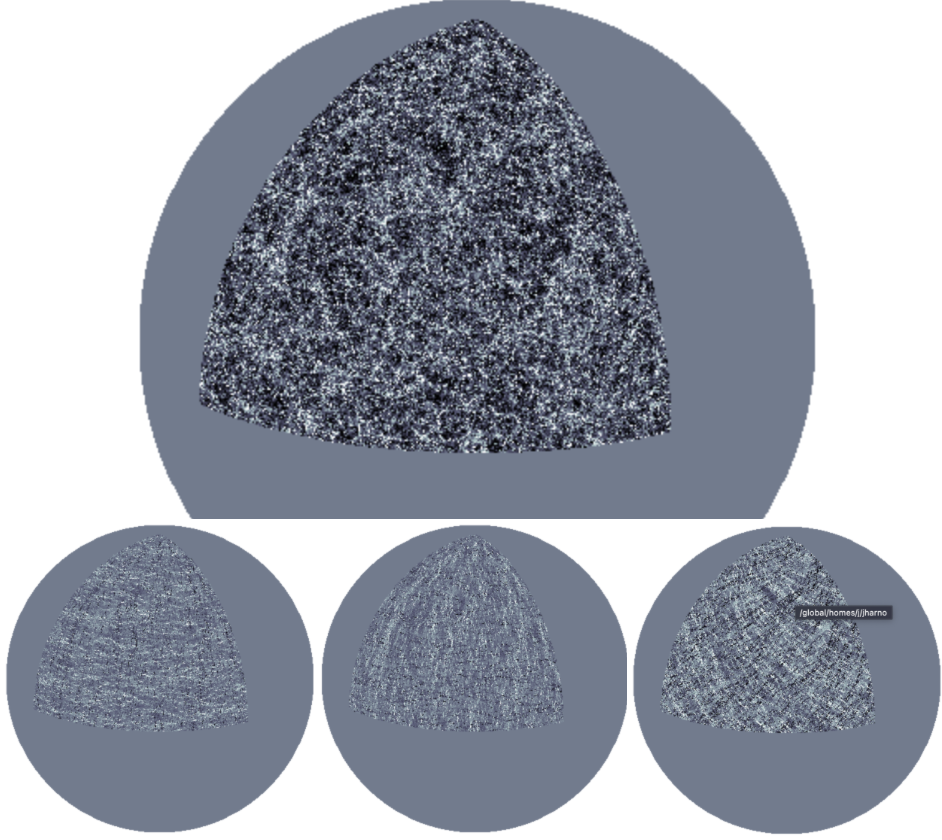
\includegraphics[width=\columnwidth]{graphs/TidalFieldOuterRim_V0}
\caption{Density field (top)  and the associated projected tidal field tensors $s_{11}$, $s_{22}$ and $s_{12}$, from left to right ({\it Improve this figure...}).}
\label{fig:maps}
\end{figure}



Our infusion method relies on couplings between intrinsic galaxy shapes and the local tidal field, hence the first step in our method consist in extracting the tidal field maps $s_{ij}(\theta,\phi)$ from the mass maps $\delta(\theta,\phi)$ that source them\footnote{Note that we have removed the redshift indexing of the maps here to simplify notation, {\it i.e.} $\delta_i(\theta,\phi) \rightarrow \delta(\theta,\phi)$.}.
In three dimensions, trace-free tidal tensor $s_{ij}(\boldsymbol x)$ can be obtained from the matter over-density field $\delta(\boldsymbol x)$ as   \citep{Catelan_IA_Tidal}:
\begin{eqnarray}
 \widetilde{s}_{ij} (\boldsymbol k)  = \left[\frac{k_i k_j}{k^2} - \frac{\delta_{ij}}{3}\right]  \widetilde {\delta}(\boldsymbol k) \mathcal{G}(\sigma_{\rm G}) \, ,
 \label{eq:sij}
\end{eqnarray}
where $\mathcal{G}(\sigma_{\rm G})$ is a three-dimensional Gaussian function described by a single (free) parameter $\sigma_{\rm G}$ that  controls the physical scales which are allowed to affect the IA term in our model. 
Tilde symbols denote Fourier-transformed quantities, the indices $(i,j)$ label the components of the Cartesian wave-vector $\boldsymbol{k}^T = (k_1,k_2,k_3)$, and $k^2 = k_1^2 + k_2^2 + k_3^2$. 
As shown in \citet{Tidalator} in the flat-sky approximation, projected tidal fields  computed from projected mass sheets provide and excellent agreement with the  theoretical NLA model, which in contrast computes the full tidal fields from the three-dimensional matter density and project along the radial dimension at the end.
We promote here this transformation to curved-sky maps, exploiting the  polarisation {\sc alm2map} operations built in {\sc Healpy}. 
In particular, noting that $Q=s_{11}-s_{22}$, $U=s_{12}$, and $\delta=s_{11}+s_{22}$, we compute the curved-sky projected  tidal field tensors ${s}_{ij}({\boldsymbol \theta})$ as:
\begin{equation}\label{eq:sij_2D_sph}
\begin{split}
    s_{11}({\boldsymbol \theta})  &=  \frac{1}{\Delta \chi_{\rm shell}}\left[\frac{ \delta + Q}{2}  - \frac{\delta}{3}\right] \\ s_{22}({\boldsymbol \theta})  &=   \frac{1}{\Delta \chi_{\rm shell}}\left[\frac{\delta - Q}{2}  - \frac{\delta}{3}\right] \\ s_{12}({\boldsymbol \theta}) &=  \frac{U}{\Delta \chi_{\rm shell}} 
\end{split}
\end{equation}
where the $U({\boldsymbol \theta})$ and $Q({\boldsymbol \theta})$ maps are smoothed by the Gaussian beam with width $\sigma_{\rm G}$, and the normalisation by  $\Delta \chi_{\rm shell}$ is required to account for the comoving thickness of the shells.
We suppress large artificial tidal fields at the boundary of our simulated octant by replicating 8$\times$ the  $\delta$ maps and carrying out these harmonic calculations  on full sky densities; we re-apply the octant mask on the tidal field maps after the last operation.
Note that the value of $\sigma_{\rm G}$ is a free parameter both in the infusion technique described in this paper and in the NLA and TATT models.
We therefore explore two cases, $\sigma_{\rm G}=0.1\mathrm{Mpc}$ and $0.5\mathrm{Mpc}$, however this may be further optimised in the future.
Finally, the full-sky density field is downgraded from $N_{\rm side}=8192$ to $N_{\rm side}=4096$ since the smoothing washes the smallest angular scales. 


%are specified within the NLA model. Smoothing amounts to selecting physical scales that do not contribute to the alignment of galaxies, which is still a debatable quantity, but is also introduced for numerical stability. \citet{Blazek2015} argues that 1.0 $h^{-1}$Mpc could be a reasonable fiducial value, being larger then the typical halo size, but recognizes that one-halo terms are also required to better match the observations. In their later work, \citet{Blazek2019} do not include smoothing at all, and neither do the KiDS-1000 nor DES-Y1 analyses based on the NLA model \citep{KiDS1000_Asgari,DESY1_Troxel}. In this work we used a two-dimensional Gaussian filter and calibrated $\sigma_{\rm G}$ empirically to $\sigma_{\rm G}=0.1h^{-1}$Mpc (see Sec. \ref{subsubsec:sigma_G}), however these two choices are arbitrary and could possibly be better optimised in the future; we also explore $\sigma_{\rm G}=0.5h^{-1}$Mpc later on.  We note that the smoothing scale is degenerate with the resolution of the simulation itself, and that one should use caution when smoothing on scales that approach the resolution limits.

%We employ a numerical technique worth mentioning here: the Fourier transforms involved in computing Eq. (\ref{eq:sij_2D}) are computed from the full (projected) periodic boxes of the simulations, then interpolated on the light-cones. We find that tidal field computed directly from the $10\times10$ deg$^2$ light-cones introduces significant large scales features in the tidal field maps, largely caused by  the non-periodic boundary conditions, which our method avoids.
Projected tidal field maps $s_{11}$, $s_{22}$, and $s_{12}$ are constructed that way for each mass sheets; Fig. \ref{fig:maps} shows the  three tidal fields and the underlying density maps for one of them.
We can clearly see the connection between all maps around over-dense regions. . 


%of every light-cones and interpolated at the position of every galaxy. Fig. \ref{fig:tidalator} illustrates this process for a small zoomed-in patch at $z\sim0$, starting from a $\delta_{2D}(\boldsymbol \theta)$ map (upper large panel), computing the tidal field components (middle four panels) and comparing the results with the cosmic shear signal generated by the same mass distribution (bottom two panels). The tidal field maps clearly reproduce the cosmic shear maps, and the minus sign in front of both terms in Eq. (\ref{eq:tidal_th}) causes the IA to undo some of the lensing signal.

\subsection{Infusion of intrinsic alignments}
\label{subsec:IA_infusion}

Having now produced shear catalogues and tidal field maps, we can use Eq. (\ref{eq:tidal_th}) to couple linearly the alignment of galaxies with the local tidal field, or Eq. (\ref{eq:tidal_th_TT}) to use instead a quadratic coupling. These allow us to compute the intrinsic ellipticities ${\boldsymbol \epsilon}^{\rm int}$ for the six IA models described in Sec. \ref{sec:IA_th}, which we combine with the cosmic shear signal ${\boldsymbol g}$ to compute observed ellipticities: 
\begin{equation}
{\boldsymbol \epsilon}^{\rm obs} = \frac{{\boldsymbol \epsilon}^{\rm int} + {\boldsymbol g}}{1 + {\boldsymbol \epsilon}^{\rm int}{\boldsymbol g^*}} 
\label{eq:eps_obs}
\end{equation}
with
\begin{equation}
{\boldsymbol \epsilon}^{\rm int}  = \frac{{\boldsymbol \epsilon}^{\rm IA} + {\boldsymbol \epsilon}^{\rm ran}}{1 + {\boldsymbol \epsilon}^{\rm IA}{\boldsymbol \epsilon^{\rm ran, *}}}.
\label{eq:eps_int}
\end{equation}
In the above expressions, the denominators ensure that the combined  ellipticities never exceed unity.
The complex spin-2 reduced shear
\begin{equation}
{\boldsymbol g} \equiv \frac{\gamma_1 + {\rm i} \gamma_2}{1 + \kappa}
\end{equation}
is computed from the shear  $(\gamma_{1/2}$) and convergence ($\kappa$) maps, interpolated at the galaxy positions and redshifts. 
The random orientation term ${\boldsymbol \epsilon}^{\rm ran}$ is drawn from two Gaussians (one per component\footnote{We further constraint  the random ellipticity to satisfy $|{\boldsymbol \epsilon}^{\rm ran}| \le 1.0$.}) with their standard deviations matching the LSST-Y1 forecast, $\sigma_{\epsilon} = 0.27$, although in most calculations we work with noise-free shapes to better resolve the IA signal.  
%We recall that since our simulated galaxy catalogues trace the dark matter density, our default IA-infusion method  is consistent with the $\delta$-NLA model (see Sec. \ref{subsec:IA_th_ext}). Analytical predictions for the two-point functions are more involved in this case \citep[see][]{Blazek2019} and not yet available on the public {\sc cosmoSIS} release. We therefore validate our methods with the standard NLA first, which we infuse by `correcting' the $\delta$-NLA measurement with Eq. (\ref{eq:tidal_th_deltaNLA}), i.e. by replacing ${\boldsymbol \epsilon}^{\rm IA}$ by ${\boldsymbol \epsilon}^{\rm IA}/(1 + b_{\rm TA} \delta)$ in our simulations. Once again, these are less realistic but better suited for validation of the measured $\gamma$-2PCFs against a theoretical model; after this is established, we use the $\delta-$NLA catalogues as our fiducial infusion model. 
%We re-iterate here that the same tidal fields, shear maps, and IA coupling equations are used for the NLA and \dNLA models, and separately for the TT and \dTT models; these only differ by the fact that in one case the galaxies are placed at random on the octant, while in the other case they are linearly tracing the dark matter.
Finally, once all galaxies have been placed in the light-cone, we interpolate the shear and IA quantities at their exact location.
Note that our current IA models make no differentiation between galaxy colours or type, and instead treats the full sample as a single population that has a single, effective, alignment signal \citep[see][for an example with a red/blue split]{DESY1_IA_Samuroff}.


